\documentclass[11pt]{article}
\usepackage{amsmath,textcomp,amssymb,graphicx,comment,tikz}
\usepackage[margin=0.75in]{geometry}
\usetikzlibrary{arrows}
\newcommand{\tab}{\hspace*{2em}}

\def\Name{Alvin Wong (22655478, -cq) , Wai Meng Lei (23985541, -dy) , Chun Yin Yau (24023460, -em)}  % Your name

\title{CS189 --- Homework 6}
\author{\Name}
\markboth{CS189 Homework 6}{CS189 Homework 6}
\pagestyle{myheadings}

\begin{document}
\maketitle

\section*{1. Single-Layer Neural Network}

\textbf{ Derivation of gradient updates: }
\\\\\
Let $y_k = \sigma ( s_k  ) $, where $s_k  = \sum_j W_{jk} x_j + b_k $.
\\\\
1) Using the mean squared error: $J = \frac{1}{2} \sum_{k=1}^{n_{out}} (t_k - y_k)^2 $:
$$ \begin{aligned}
\frac{dJ}{d W_{jk} } &= \frac{d}{d W_{jk}} ( \frac{1}{2} \sum_{k=1}^{n_{out}} (t_k - y_k)^2 \\
&= (y_k - t_k) \frac{d}{d W_{jk}} \sigma(s_k) \\
&= (y_k - t_k) \sigma(s_k) (1 - \sigma(s_k)) \frac{d}{d W_jk} (W_{jk} x_j + b_k) \\
&= (y_k - t_k) \sigma(s_k) (1 - \sigma(s_k)) x_j 
\end{aligned} $$
$$ \begin{aligned}
\frac{dJ}{d b_j } &= \frac{d}{d b_j} ( \frac{1}{2} \sum_{k=1}^{n_{out}} (t_k - y_k)^2 \\
&= (y_k - t_k) \frac{d}{d b_j} \sigma(s_k) \\
&= (y_k - t_k) \sigma(s_k) (1 - \sigma(s_k)) \frac{d}{d b_j} (W_{jk} x_j + b_k) \\
&= (y_k - t_k) \sigma(s_k) (1 - \sigma(s_k)) 
\end{aligned} $$
In terms of matrices and vectors:
Let $\vec{y} = \sigma ( \vec{s} )$, and $\vec{s} = W \vec{x} + \vec{b} $:
$$ \boxed{\frac{dJ} {dW} = diag(\vec{y}) (1 - diag(\vec{y})) [ \vec{y} - \vec{t} ] \vec{x}^T} $$
$$ \boxed{\frac{dJ} {d\vec{b}} = diag(\vec{y}) (1 - diag(\vec{y})) [ \vec{y} - \vec{t} ]} $$
2) Using the cross-entropy error: $J = - \sum_{k=1}^{n_{out}} [t_k \ln y_k + (1 - t_k) \ln (1 - y_k)] $:
\\\\
The math works out the same, it's just the initial $y_k - t_k$ term becomes the derivative of the cross-entropy error term above:
$$ \frac{dJ}{d W_{jk} } = [ - \frac{t_k}{y_k} + \frac{1 - t_k}{1 - y_k} ] \sigma(s_k) (1 - \sigma(s_k)) x_j $$
$$ \frac{dJ}{d b_j } = [ - \frac{t_k}{y_k} + \frac{1 - t_k}{1 - y_k} ] \sigma(s_k) (1 - \sigma(s_k)) $$
\newpage

\section*{1. Single-Layer Neural Network (continued)}
In terms of matrices and vectors:
$$ \boxed{\frac{dJ} {dW} = diag(\vec{y}) (1 - diag(\vec{y})) [ - \frac{\vec{t}}{\vec{y}} + \frac{ 1 - \vec{t}}{1 - \vec{y}} ] \vec{x}^T} $$
$$ \boxed{\frac{dJ} {d\vec{b}} = diag(\vec{y}) (1 - diag(\vec{y})) [ - \frac{\vec{t}}{\vec{y}} + \frac{ 1 - \vec{t}}{1 - \vec{y}} ]} $$
\textbf{Training and Testing:}
In our training algorithm, we batched the training data into minibatches of size 200, computed the gradient over all 200 of these samples, and for each batch, ran SGD to update the parameters (we update our parameters by walking in the direction of the steepest downward descent, and the step size is controlled by $\alpha$). Our initial value of $\alpha$, the learning rate, was 0.01. We used the decay function $$ -1 / (1 + exp(-10t / n)) + 1 $$ which is a decaying function, but the decay starts off much more slower than a regular 1/t decay function.
\\\\
\textbf{Figure 1: Plot of the training loss (blue) and test set accuracy (red), 500 epochs, MSE error}  \\\\
The test accuracy converged to 92.25\%. The total training loss converged to about 4370. This took about a little over two hours to run. (About 4 epochs per minute). To run the code, run singleNNBenchmark(false).
\\
\begin{figure}[ht!]
\centering
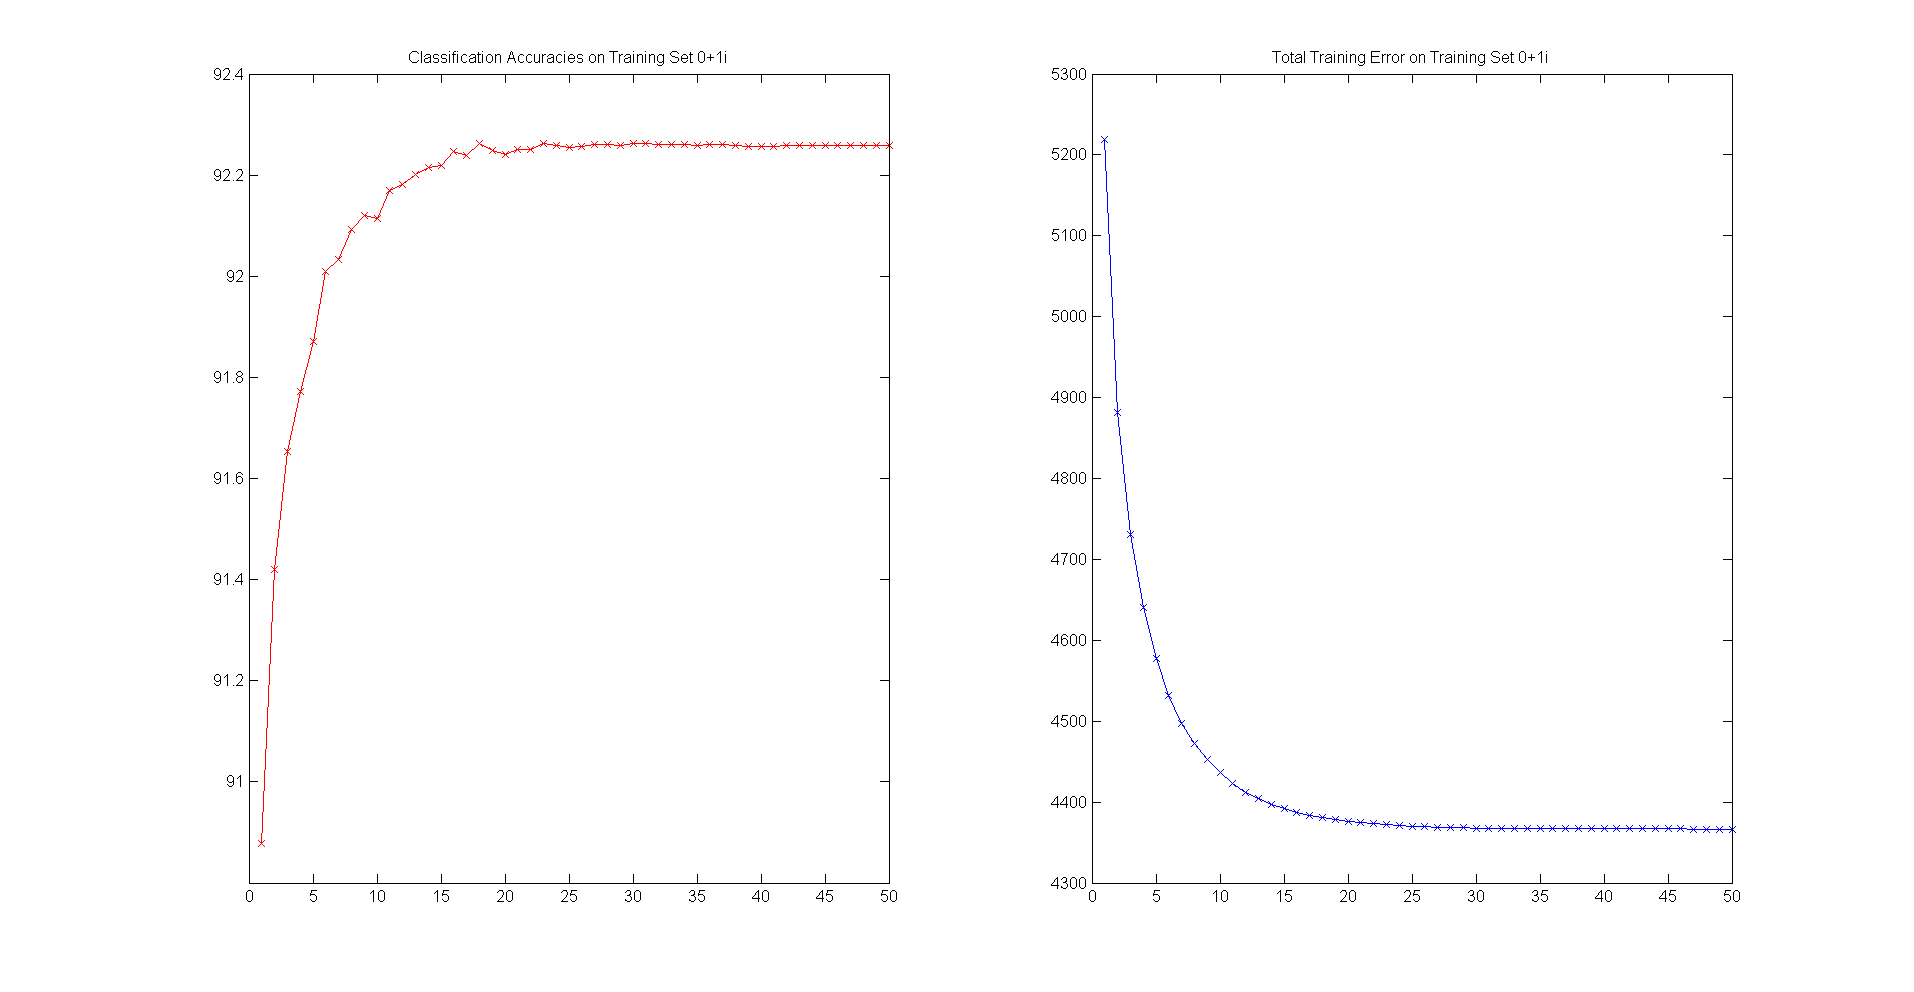
\includegraphics[width=180mm]{plots/finalp1mse.png}
\label{overflow}
\end{figure}
\\
Note: don't mind the titles -- they are wrong. Left graph is on test accuracy. Right graph is on training set loss.
\\
\newpage
\section*{1. Single-Layer Neural Network (continued)}
\textbf{Figure 2: Plot of the training loss (blue) and test set accuracy (red), 500 epochs, CE error} \\
The test accuracy converged to 92.8\%. The total training loss converged to about 34300. This took about a little over two hours to run. (About 4 epochs per minute). To run the code, run singleNNBenchmark(true).
\\
\begin{figure}[ht!]
\centering
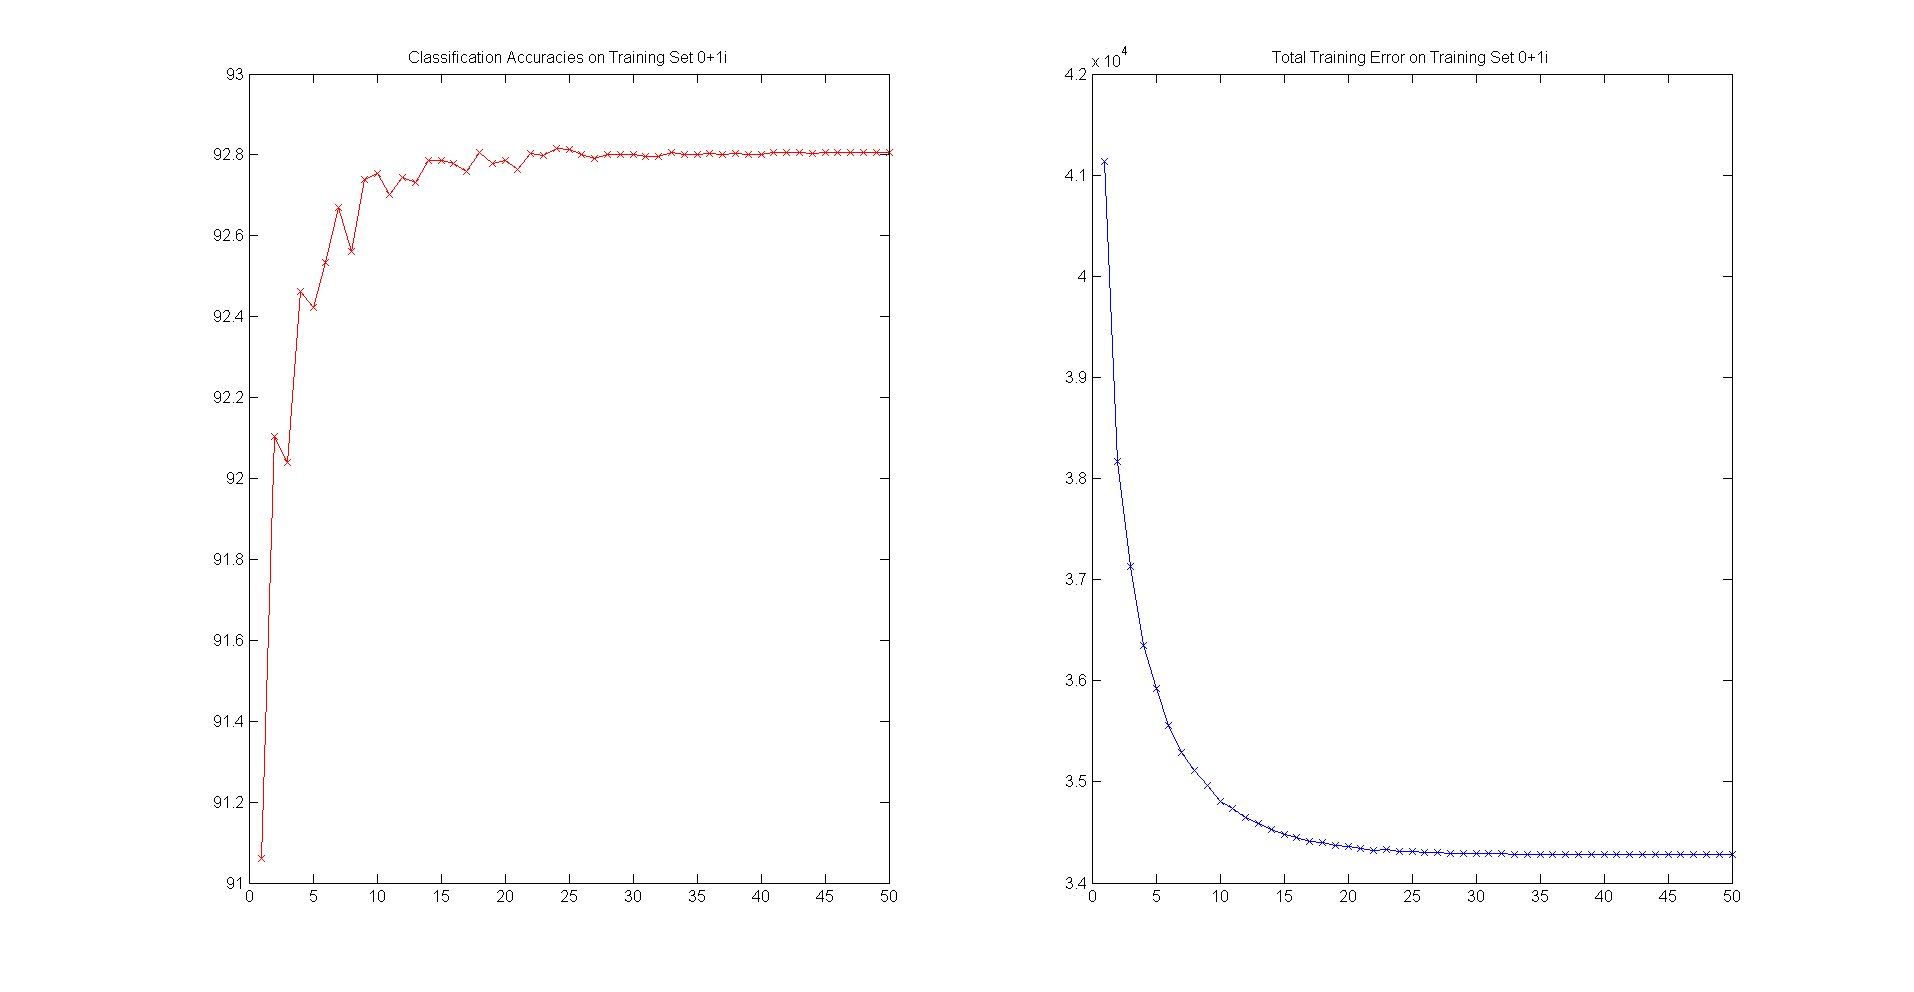
\includegraphics[width=180mm]{plots/finalp1ce.png}
\label{overflow}
\end{figure}
\\
Note: don't mind the titles -- they are wrong. Left graph is on test accuracy. Right graph is on training set loss.

\section*{2. Multi-Layer Hidden Neural Network}
\textbf{ Derivation of gradient updates:}
\\\\
We'll be making use of the previous question's derivations to help us here:
\\\\
1) Using the mean squared error: $J = \frac{1}{2} \sum_{k=1}^{n_{out}} (t_k - y_k)^2 $:
\\\\
Note: might have flipped the dimensionalities of the matrices, but nevertheless it's just a transpose difference.
\\\\
Let: \\
$ \vec{s_1} = W_1 \vec{x} + \vec{b_1} $ \\
$ \vec{s_2} = W_2 tanh(\vec{s_1}) + \vec{b_2} $ \\
$ \vec{s_{out}} = W_{out} tanh ( \vec{s_2}) + \vec{b_{out}} $ \\
$ \vec{y} = \sigma (\vec{s_{out}}) $
\\\\
(continued on next page)
\newpage

\section*{2. Multi-Layer Hidden Neural Network (continued)}
Then the backprop algorithm works as follows: \\
$ \vec{\delta_{out}} = diag(\vec{y}) diag(1 - \vec{y}) [ \vec{y} - \vec{t}] $ \\
$ W_{grad, out} \leftarrow W_{grad,out} + \vec{\delta_{out}} tanh(\vec{s_2})^T $ \\
$ b_{grad, out} \leftarrow b_{grad,out} + \vec{\delta_{out}}  $ \\
$ \vec{\delta_2} = (1 - tanh(\vec{s_2})^2) .* W_{out}^T \vec{\delta_{out}} $ \\
$ W_{grad, 2} \leftarrow W_{grad,2} + \vec{\delta_{2}} tanh(\vec{s_1})^T $ \\
$ b_{grad, 2} \leftarrow b_{grad,2} + \vec{\delta_{2}} $ \\
$ \vec{\delta_1} = (1 - tanh(\vec{s_1})^2) .* W_{2}^T \vec{\delta_{2}} $ \\
$ W_{grad, 1} \leftarrow W_{grad,1} + \vec{\delta_{1}} tanh(\vec{x})^T $ \\
$ b_{grad, 1} \leftarrow b_{grad,1} + \vec{\delta_{1}} $ \\
\\\\
We'll then apply SGD with a time varying $\alpha$ rate to update the parameters by the gradients.
\\\\
2) Using the cross-entropy error: $J = - \sum_{k=1}^{n_{out}} [t_k \ln y_k + (1 - t_k) \ln (1 - y_k)] $:
\\\\
The math works out the same, it's just the initial $\vec{y} - \vec{t}$ term becomes the derivative of the cross-entropy error term above:
\\\\
Then the backprop algorithm works as follows: \\
$ \vec{\delta_{out}} = diag(\vec{y}) diag(1 - \vec{y}) [ - \frac{\vec{t}}{\vec{y}} + \frac{ 1 - \vec{t}}{1 - \vec{y}} ]$ \\
$ W_{grad, out} \leftarrow W_{grad,out} + \vec{\delta_{out}} tanh(\vec{s_2})^T $ \\
$ b_{grad, out} \leftarrow b_{grad,out} + \vec{\delta_{out}}  $ \\
$ \vec{\delta_2} = (1 - tanh(\vec{s_2})^2) .* W_{out}^T \vec{\delta_{out}} $ \\
$ W_{grad, 2} \leftarrow W_{grad,2} + \vec{\delta_{2}} tanh(\vec{s_1})^T $ \\
$ b_{grad, 2} \leftarrow b_{grad,2} + \vec{\delta_{2}} $ \\
$ \vec{\delta_1} = (1 - tanh(\vec{s_1})^2) .* W_{2}^T \vec{\delta_{2}} $ \\
$ W_{grad, 1} \leftarrow W_{grad,1} + \vec{\delta_{1}} tanh(\vec{x})^T $ \\
$ b_{grad, 1} \leftarrow b_{grad,1} + \vec{\delta_{1}} $ 
\\\\
\textbf{Testing and Training:}
\\\\
In our training algorithm, we batched the training data into minibatches of size 200, computed the gradient over all 200 of these samples, and for each batch, ran SGD to update the parameters (we update our parameters by walking in the direction of the steepest downward descent, and the step size is controlled by $\alpha$). Our initial value of $\alpha$, the learning rate, was 0.01, for the MSE error loss function. For the CE loss function, we started with a smaller step size: $\alpha = 0.004$. We used the decay function $$ -1 / (1 + exp(-5t / n)) + 1 $$ which is a decaying function, but the decay starts off much more slower than a regular 1/t decay function. We used the two error functions and have functional code working for both.
\newpage
\section*{2. Multi-Layer Hidden Neural Network (continued)}
\textbf{Figure 3: Plot of the training loss (blue) and test set accuracy (red), 150 epochs, MSE error}  \\\\
The test accuracy converged to 97.07\%. The total training loss converged to about 1110. This took about a little over 6 hours to run. (About 1 epoch per 2.5 minutes). To run the code, run multiNNBenchmark(false).
\\
\begin{figure}[ht!]
\centering
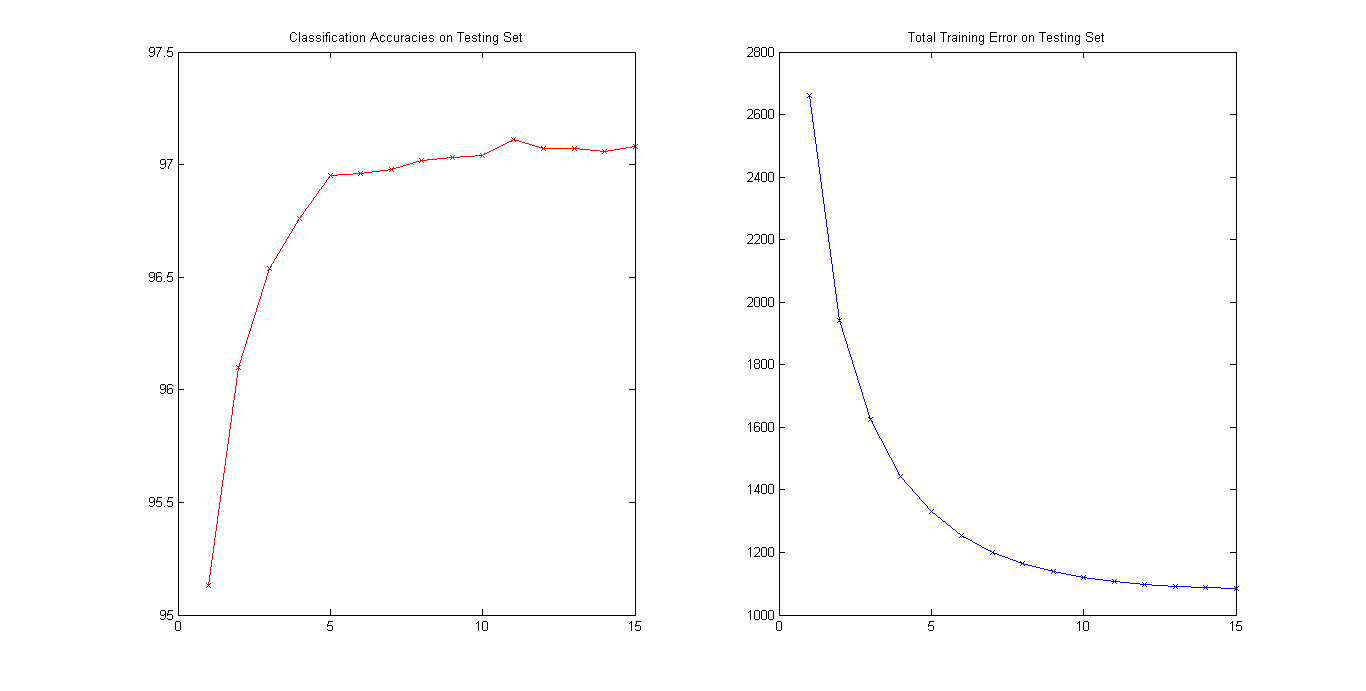
\includegraphics[width=180mm]{plots/finalp2mse.png}
\label{overflow}
\end{figure}
\\
(continued on next page)
\newpage
\section*{2. Multi-Layer Hidden Neural Network (continued)}
\textbf{Figure 4: Plot of the training loss (blue) and test set accuracy (red), 60 epochs, CE error} \\\\
The test accuracy converged to 97.08\%. The total training loss converged to about 7980. This took about a little over 2.5 hours to run. (About 1 epoch per 2.5 minutes). To run the code, run multiNNBenchmark(true).
\\
\begin{figure}[ht!]
\centering
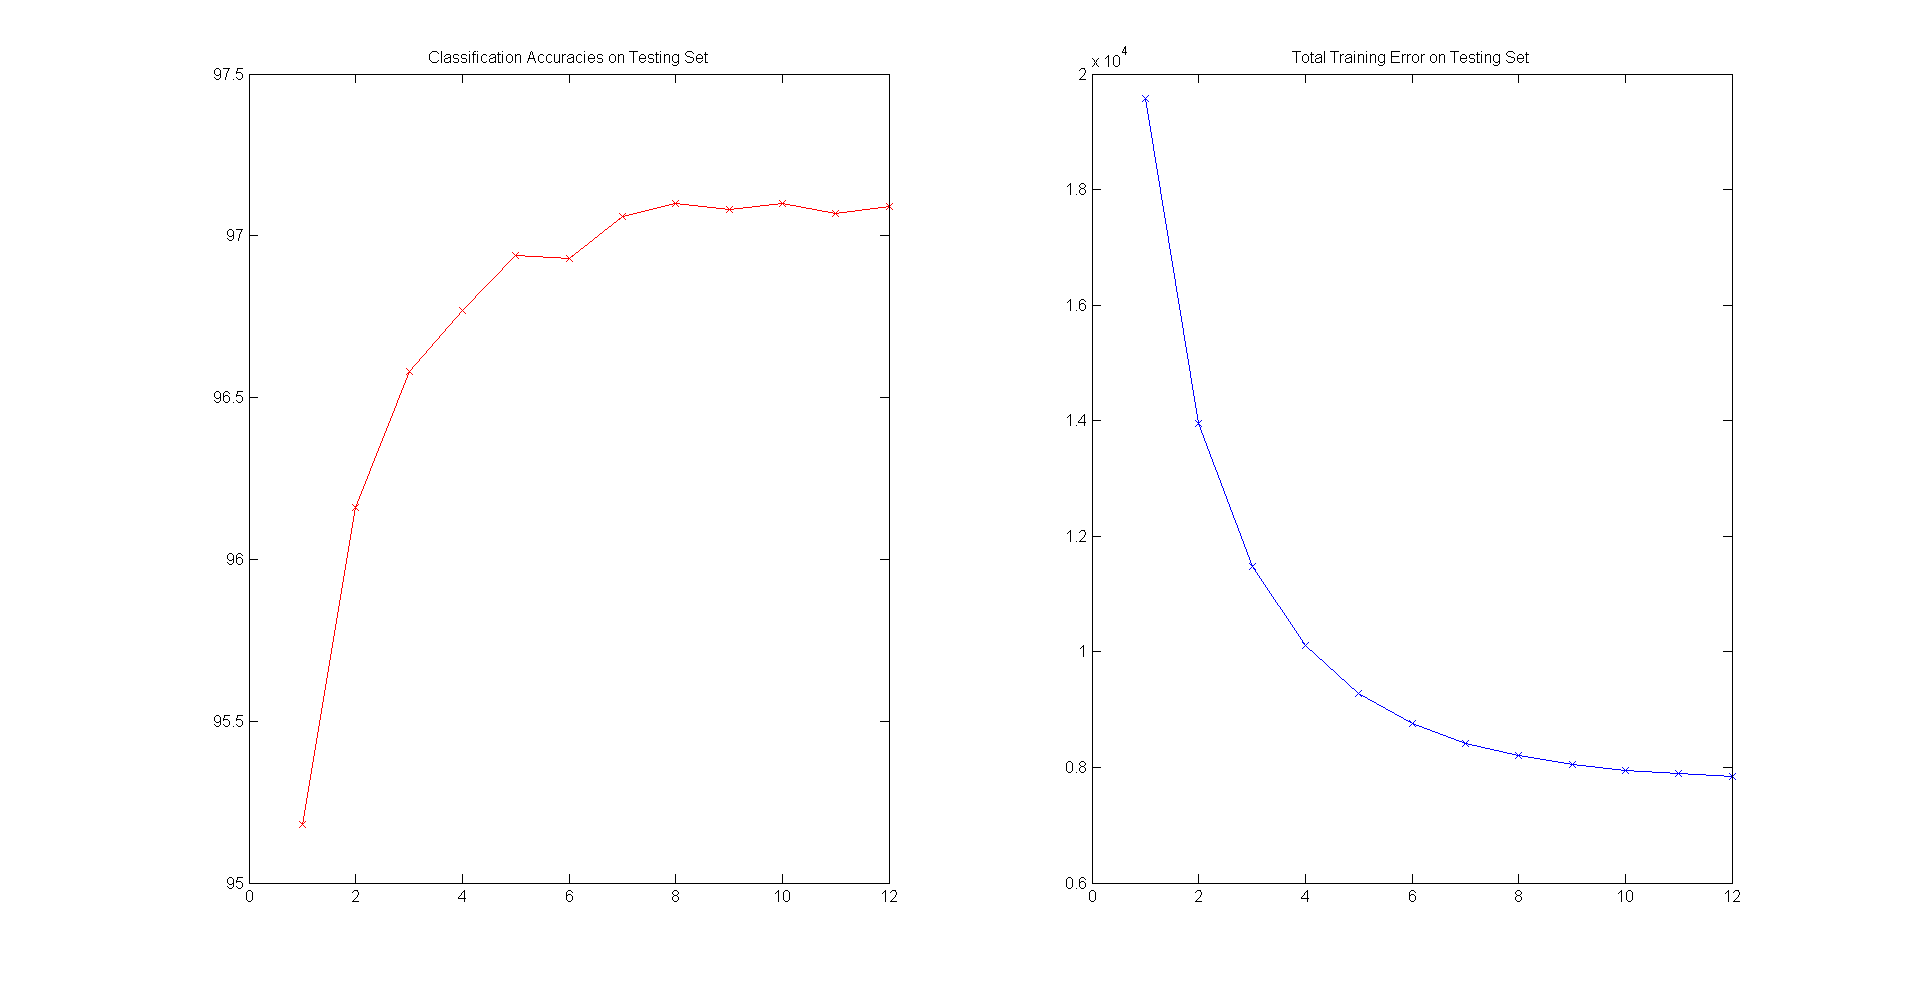
\includegraphics[width=180mm]{plots/finalp2ce.png}
\label{overflow}
\end{figure}





\end{document}
